\documentclass[]{article}
\usepackage[colorinlistoftodos]{todonotes}
%For front page purposes
\usepackage{pdfpages}
%MISC
\usepackage{framed}
\usepackage{hyperref}
\usepackage{url}
% To handle Icelandic letters
\usepackage[utf8]{inputenc}
\usepackage[T1]{fontenc}


%opening
\title{Like Breeder\\ \small Report in the course Procedural Content Generation in Games, Autumn 2014}
\author{Björn Þór Jónsson - \texttt{bjrr@itu.dk}\\Kasper Fryland Appeldorff - \texttt{kfap@itu.dk}}

\begin{document}
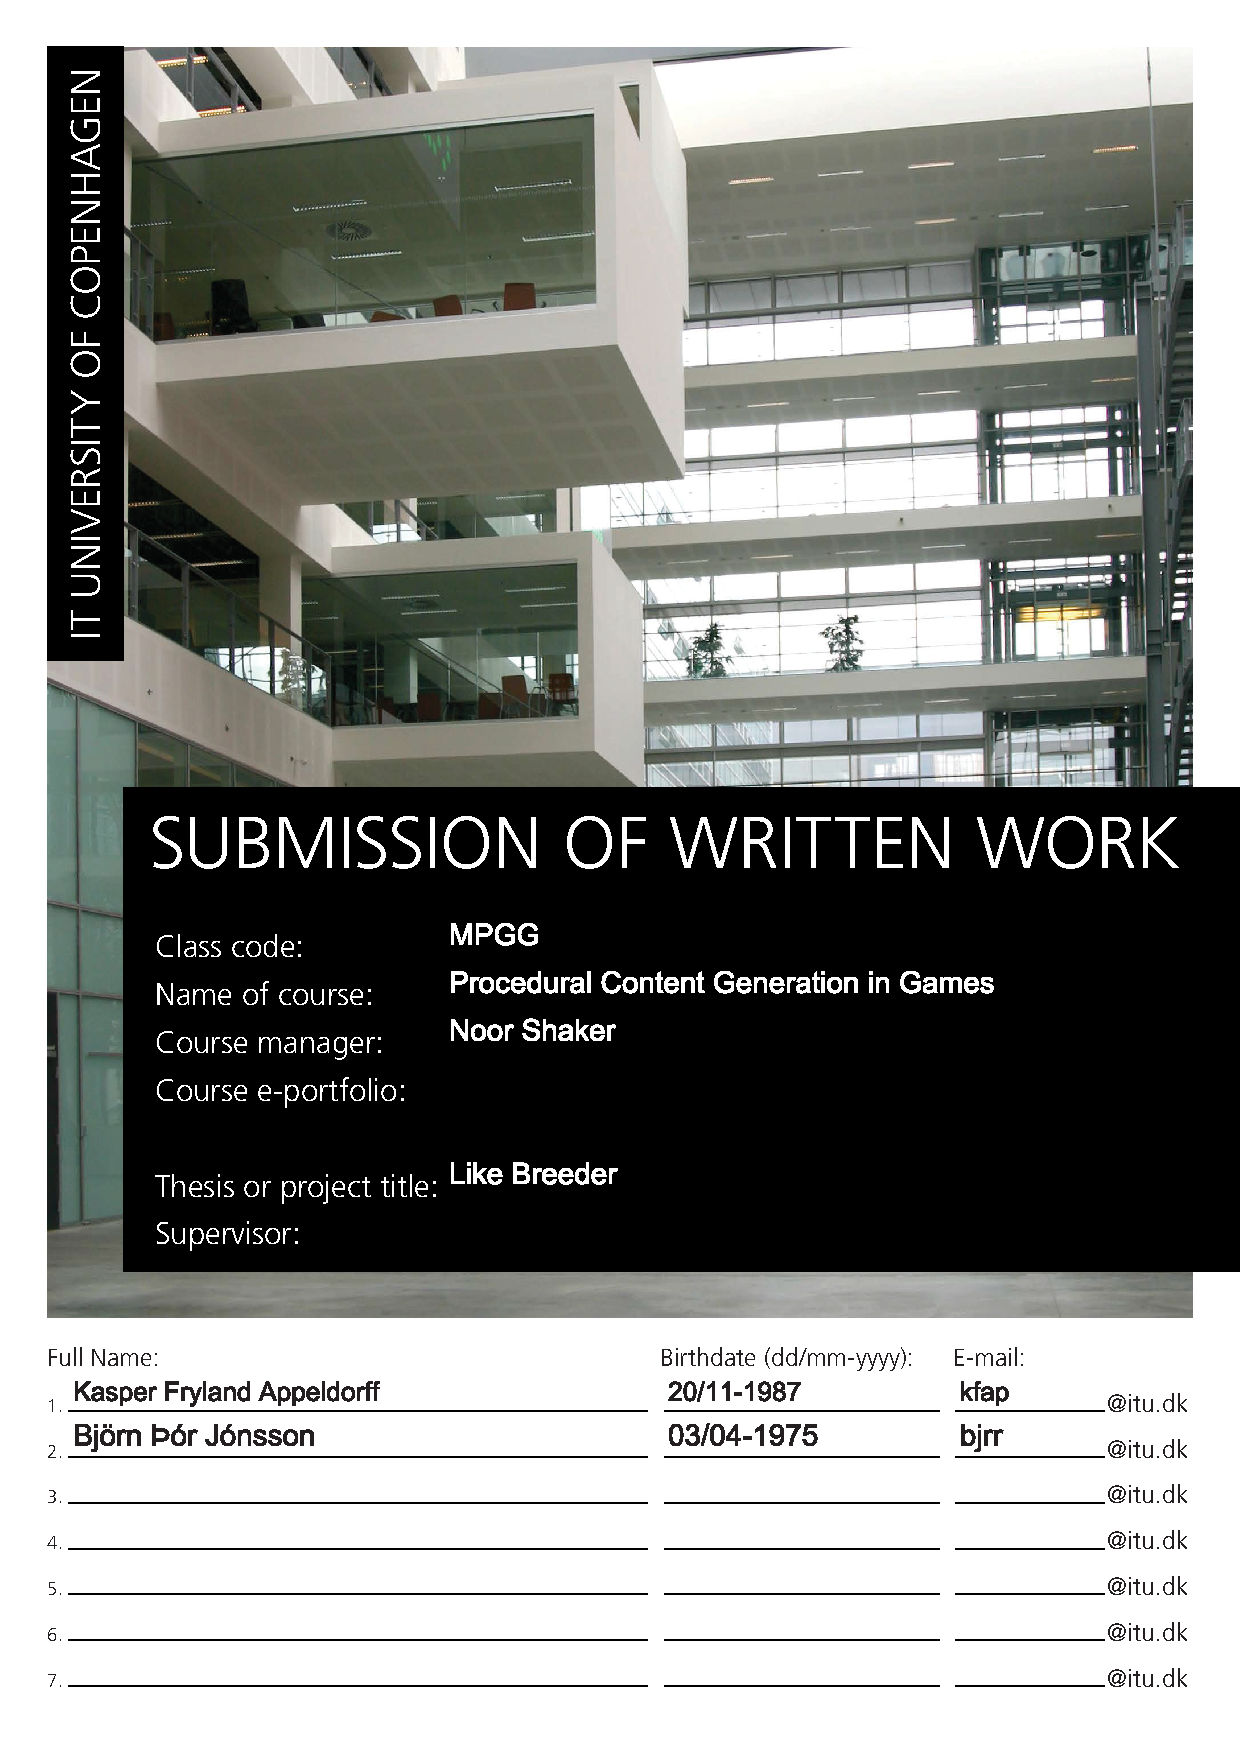
\includepdf{frontpage.pdf}
\maketitle
%\tableofcontents %Table of contents. Automagic
%\listoffigures %Also has \listoftables
\listoftodos % Requires package todonotes
\newpage
\begin{abstract}
\todo[color=red]{Put summary here}
\end{abstract}

\section{Introduction}
\label{sec:Introduction}
\begin{framed}
What problem are you trying to solve?Why is this important? How does this problem make some sort of game better?
\end{framed}

\begin{itemize}
\item Social media is incredibly popular. Facebook has 1.35 billion active users in November 2014 (\url{http://www.statista.com/statistics/272014/global-social-networks-ranked-by-number-of-users/} Need stupid free acct to see the source but we can deal with that later)
	\begin{itemize}
	\item Tumbler had 230 million in that month - same source
	\end{itemize}
\item A lot of content is shared on social media . images, gifs, videos, text etc (citation for amount would be great)
\item Games have become a large part of social media (citation needed)
\item Noone has turned the content on social media into a game.
\item In this paper we will introduce, discuss etc a concept for a game on social media with content provided by social media
\end{itemize}



\section{Background}
\label{sec:Background}

\begin{framed}
Has this been done before? How? If not, what’s the closest related research? (Both using similar approaches and other algorithms.) What’s novel with your research?
\end{framed}

\begin{itemize}
\item Has not been done before. Using social media content for games is novel in itself.
	\begin{itemize}
	\item We might want to look in to what others have done with tags (which we probably should have done to begin with), so we can place ourselves somewhere on some sort of spectrum
	\end{itemize}
\item I suppose what is novel is that it has not been done before heh
\end{itemize}

...other related work
\todo{racing tracks article, picbreeder article}

\todo{check What Makes People Click article, and others...}



\section{Game Design}
\label{sec:GameDesign}

How does this relate to games?  Rating those sets of media items, with the aim of creating cubes representative of one's person, can be looked upon as a form of play, whereas games in general are one form of play.  It can be categorized as an Alea play form \cite{caillois2001man}, with a resemblance of playing a slot machine, though less random in nature while appealing to personal interests.  The cubes bred in this playful activity an can then be considered as play / game content, that can be brought by their creator into various playful activities.  With the option of 3D printing the cubes, they could become tangible toys, fit for play and games in the physical reality.

An example of a game to play, with such like-cubes, can be a quiz where two opponents are each presented with a set of three media-items-cubes and are to guess which one was created by their opponent.  Two of the cubes presented to each player are either randomly generated, selected from other user's collections, or assembled with selection based on heuristics obtained from the imported social media sites activity for each participating player, and one cube is chosen from the collection of cubes she has actually created.  Scores are given for each correct guess and players compete to become experts in each other's likes.  Such play can be viewed purely as a pastime or as a way for people to get to know each other.  Games like \textit{Guess Who?}\cite{GuessWho} can be compared to this quiz example and even inspire further elaborations on it.

Among other conceivable examples is an environment where players assemble with their cube selections, with the aim of arranging them in creative ways into strings of narratives, were short text fragments connect the cubes along interesting storylines (Figure~\ref{fig:narratives}).  Players would vote on the assembled narratives and possibly compete at receiving the most likes on their creations (Fig TODO: Photograph of cubes at play).  More examples of play with social media items can be conceived and a collection of possible play scenarios can be seen in \cite{GoLplay}.

\begin{figure}[htp]
	\missingfigure{photo of like cubes arranged in strings of narratives.}
	\caption{Paper prototype of like-cubes at play in the creation of different narratives.}
	\label{fig:narratives}
\end{figure}

Assembling media content from ones collection of likes and posts from social media websites, by manually scanning through the items in a linear fashion, would likely be perceived as tedious work.  Aiding that activity with a variant of \textit{procedural} evolution, \textit{generating content} for social media games in a playful fashion, could increase the odds of potential players becoming engaged in that process.


\begin{framed}
What’s the design of the game you are going to use? Why do you need PCG in this game?
\end{framed}
\begin{itemize}
\item \href{Guess who}{http://boardgamegeek.com/boardgame/4143/guess-who} - sort of. Presented with cubes (similar cubes) - some from strangers, at least one from a friend. Guess which cube is your friend.
\item Story mode - Connect images on a cube to a story
\item Got more?
\end{itemize}
\todo{examples of games the cubes can be used in}

\todo{cite article on importance of avatar creation for players}



\section{Methods}
\label{sec:Methods}

This project is inspired by the article \textit{Interactive Evolution for the Procedural Generation of Tracks in a High-End Racing Game} \cite{cardamone2011interactive}.  Content presentation and user interaction is based on the discussion in that article and the related project.  Instead of composing tracks for a racing game, the aim here is to breed sets of media items that a participant finds representative of her as a person.


\subsection{Initial Genetic Algorithm design}

Having supplied user handles for various social media networks to the like-breeding system, a participant is presented with a population created from a random selection of social media items she has posted or liked on the chosen networks.  In the prototype discussed in this report, access to only one network is implemented:  Tumblr.

The initial idea was to have individuals in this population composed as sets of media items, four or six in each set, and have the participant rate how well each set represents her as a person.  Then a new generation would be evolved, based on the ratings of individuals in the previous generation.  For the Genetic Algorithm, the \textit{phenotype} would be composed of the four or six media items, for decorating the sides of the “personality cube”.  
The \textit{genotype} would be an array of length four or six, of which each element is another array of tags, or if no tags accompany a media item, then the element would simply be the media item's ID / URL.
\textit{Reproduction} could be based on a crossover from the sequences of tag sets / media IDs from the parents.  
Elements in the genes of children could be copied directly from the parents or be populated with tags from new media items found in searches by the tags found in parent elements.

\begin{figure}[htp]
	\missingfigure{photo of like cubes arranged in strings of narratives.}
	\caption{Initial mockups of UI screens showing among other things, like-cube breeding with Interactive Evolutionary Computation, where each individual is a set of media items, and ratings are applied to each individual set.}
	\label{fig:breedingMockup}
\end{figure}


\subsection{Simplification resulting in a deviation from traditional genetic evolution}

After receiving feedback from a potential user of the breeding system, that was not involved in the project implementation, concerning the complexity of digesting multiple sets of media items at a time from one population, a decision was taken to simplify the user interface.  In an effort to lessen user fatigue, the interface was redesigned to show only one set of media items at each evolution step.  That simplified version resembles slot machines or bandits and that familiarity can be considered as an asset.  The resemblance stems especially from the change of interaction, from applying ratings to item sets to that of holding the preferred items in each given set and rolling the rest to evolve the next generation (Figure~\ref{fig:likeBreeder}).

\begin{figure}[htp]
	\missingfigure{Like-Breeder screen shot.}
	\caption{Screen shot of the Like Breeder prototype, with the simplified interface only showing one set of media items at a time.}
	\label{fig:likeBreeder}
\end{figure}

A result of this redesign is that our breeding algorithm has to deviate from the traditional progression of Genetic Algorithms, as there is now only one individual in the population and evaluation of fitness among individuals, selection and mating, does not apply.  As there is just the equivalent of one cube on display at a time, to lessen user fatigue, instead of many as was originally planned, there is no evolution among competing individuals.  Competition happens now among individual genes, the media items, to get a seat within the genome of that one individual.  Now there is competition among genes, rather than genotypes.


...\todo{Kasper, could you do a write up on some of the bullets here?  ...distance measures, Jaccard vs. Euclidean... "explain why various ways of not searching the entire space doesnt work"... etc.)}


\subsection{Suitable platforms}

Games played with social media items, such as the examples discussed in this report, fit naturally within web browser environments and are less suitable for the more traditional game engine technologies, such as those provided with Unity [ref to Unity answers], where it is more difficult to integrate online media content.  Such games could be played on mobile devices or desktop computers, running web browsers, among players geographically separated.  

To join people together, who are in the same place at the same time, in play with media items, a console gaming experience could be implemented for a web enabled device such as Chromecast \cite{ChromecastGames}, where players are joined in front of a common television screen, with game controls implemented for their mobile devices.  This would be more difficult to achieve on traditional living-room game consoles, such as the PlayStation, which do not not speak the language of the web naturally.



\begin{framed}
How does your algorithm work? Describe in as much detail as you can fit into the report. Classify your algorithm according to the taxonomy in the “Search-based Procedural Content Generation” paper. Also, how did you interface it to the game?
\end{framed}



\begin{itemize}
\item Brief walkthrough of our method
	\begin{itemize}
	\item Why Jaccard and not Euclidean distance? Because for Euclidean we need to know what tags are there. That changes pretty often when we load async. That would require us to do a fuckload of indexOf to some taglist all the time and keep it in localStorage or generate it lots of times. Not only that but we would also start to suffer from the curse of dimensionality (citation needed), so all itemsets will appear close simply because neither of them have 90\% of tags in the list.
	\end{itemize}
\item Introduce evolution as possibly valid method
\item Discuss why evolution might be a bad choice
	\begin{itemize}
	\item If you only show one individual - how can you evaluate an entire population?
	\item If the user picks a rare gene and thereby fixes it - All children will have this particular gene and possibly more from the parent with the rare gene - this establishing a close relationship among a small group of individuals - Image 1 person with blue eyes. If blue eyes is fixed then only that 1 individual and subsequent children will have blue eyes. If they share even more traits/genes then the user could quickly and unknowingly converge.
	\end{itemize}
\item Discuss more alternatives (we might have to look into stuff about bag of words or other approaches to text analysis)
\item Also mention that speed is fast. We might want to see if we can reach over 100k by combining blogs
\end{itemize}
\todo{discuss our reasons for not really doing a proper evolution}
Suggestion from Noor:

Rather than scanning the full search space each time, initially create a n sets of images randomly.  When you have chosen to hold one or more images, find the best matching set from those n, as a part of a fitness function, and mate that set with the currently visible set.  Then do mutation by randomly selecting images from the whole space, by some chance p.


Con ->  Can reach a local optimum very quickly:  After two have been mated, the fittest individuals according the new offspring would comprise a very limited search space?

Pros ->  Limits the search space:  Won’t have to scan all images each time.

Maybe we are not evolving anything?  Then make that point.

--> Really how our evolution proceeds:\\
Pop size: 1\\
Gene = Image\\
Genome = Cube / Image set\\
Crossover = Similar\\
Mutate = Random
\todo{mention that speed is not an issue!  cite examples...}

\section{Results}
\label{sec:Results}
\begin{framed}
Did it work? How well? Provide some figures, and a table or two. How much time does it take?
\end{framed}
\begin{itemize}
\item It is fairly quick to reach a conclusion ie. a cube. User fatigue does not become an issue, not even close. Perhaps fiddle with set size?
	\begin{itemize}
	\item Timing a few runs with test subjects might be good. We sorta know how this works and as such we are rather quick.
	\end{itemize}
\item We should come up with some metrics - A lot of these are going to be subjective I fear.
\end{itemize}



\section{Discussion}
\label{sec:Discussion}


\begin{framed}
What are the strengths and shortcomings of your method? How well would it generalize to other game genres? How controllable is it, and what is the potential for using to adapt content to individual preferences? How would you develop it further, if you had time?
\end{framed}
\begin{itemize}
\item Shortcomings and strengths:
	\begin{itemize}
	\item Shortcoming: Not very advanced - We essentially use a matrix of indices
	\item Shortcoming: Pretty close to deterministic - Removes a bit of ``cool factor'' in my opinion. More of a subjective shortcoming but there it is. Not sure how we could ``fix'' this.
	\item Advantage: Does not ignore anything. When you get something back everything has been considered. No estimations etc.
	\item Advantage: Speed. Even with a large quantity of content updates are seemingly instant. Perhaps use this as an argument for not trying to reduce search space?
	\end{itemize}
\item  It seems very controllable to me. It depends on the amount of ``crap tags'' you put on your things but you can say that about any dataset - low quality data $\Rightarrow$ low quality results. 
\item Potential for individual preferences? Perhaps a dial or something for image set size. Other than that it is pretty customizable. You don't even need to have content you like - as long as you know where you can find it.
\item I would still look into some way of ``surprising'' the user. Instead of random/similar maybe finding dissimilar instead of random? Work under the assumption that not held / not similar means something different than what is there.

\item Establishing relationships between tags or other associated descriptive words, could be helpful.  Semantic relationships, rather than the Jaccardian distances currently employed.  How can they be found?  Could something like ConceptNet help in that regard?  http://conceptnet5.media.mit.edu  

\end{itemize}



\section{Readings}
Inspiration or papers with important points to make:
\begin{itemize}
\item \href{http://julian.togelius.com/Togelius2011What.pdf}{What is Procedural Content Generation? Mario on the borderline}
\item \href{http://delivery.acm.org/10.1145/1840000/1835484/p194-guy.pdf?ip=130.226.142.243&id=1835484&acc=ACTIVE\%20SERVICE&key=36332CD97FA87885\%2E6A18944DEFDDF4C0\%2E4D4702B0C3E38B35\%2E4D4702B0C3E38B35&CFID=605494385&CFTOKEN=58221236&__acm__=1417798342_c9dde7c05e2a19158dcc16e124ca0723}{Social Media Recommendation based on People and Tags }
\end{itemize}

\bibliographystyle{unsrt}
\bibliography{references}
\end{document}
